\chapter{Fundamentação Teórica}
\label{cap:fundamentacao-teorica}

Este capítulo reúne os conceitos filosóficos e computacionais que sustentam a pesquisa. A primeira parte discute diferentes concepções de inteligência e apresenta noções relacionadas à vida, à autonomia, à autopoiese e à perspectiva enativa. A segunda parte aborda os fundamentos do Aprendizado por Reforço e do Aprendizado por Reforço Profundo, incluindo métodos de otimização de políticas, motivação intrínseca, curiosidade artificial e técnicas de análise visual das políticas aprendidas.

\section{Fundamentação Filosófica}

\subsection{Inteligência Como Resolução de Problemas}

A palavra inteligência vem do latim \textit{intelligentia}, derivada do verbo intelligere (\textit{inter}, ``entre'' e \textit{legere}, ``escolher'', ``colher'', ``separar'', ``ler'').  Portanto, em sua origem, inteligência significa a capacidade de escolher entre várias opções ou, mais profundamente, ``ler entre'' (as linhas, os fatos, as aparências). Não é apenas processar o que está lá, mas discernir o que é relevante e o que não é.

Entretanto, na Inteligência Artificial(IA) atual, a concepção de ``inteligência'' é frequentemente reduzida a resolução de problemas, tarefas específicas, otimização ou desempenho em benchmarks, em detrimento de aspectos mais amplos da inteligência humana, como compreensão profunda, criatividade ou raciocínio contextual. A IA atual demonstra mais ``conquista artificial'' (conquistas em tarefas específicas) do que inteligência genuína, pois é limitada a problemas treinados, sem capacidade de resolver problemas novos como humanos. \cite{bridging-the-gap}.

Um dos maiores e mais famosos exemplos desta concepção de inteligência pode ser vista em \citeonline{turing1950computing}. Nesse texto, Alan Turing propõe uma reformulação da pergunta clássica ``As máquinas podem pensar?'' para evitar debates semânticos sobre os termos ``máquina'' e ``pensar''. Em vez de definir diretamente o que é inteligência, ele introduz o jogo da imitação, hoje conhecido como Teste de Turing. No teste, um interrogador humano conversa por texto, sem ver ou ouvir os interlocutores, com dois participantes: um humano e uma máquina. O objetivo é determinar se a máquina consegue imitar respostas humanas de forma tão convincente que o interrogador não consiga distinguir qual é a máquina. Se a máquina passar no teste, Turing sugere que seria razoável dizer que ela ``pensa'' ou exibe inteligência. Todavia, o Teste de Turing  representa o início da visão contemporânea de inteligência, baseada em resolução de problemas específicos previamente definidos, como responder perguntas de forma indistinguível de um humano, sem exigir ``leitura entre as linhas'' (\textit{intelligere}) ou consciência, sendo o ``Argumento do Quarto Chinês'' \ \cite{searle1980minds} o principal argumento a favor disto.

O ``Argumento do Quarto Chinês'' propõe um cenário hipotético destinado a ilustrar que a manipulação sintática (símbolos), por si só, não produz compreensão semântica (significado). Imagine uma pessoa que não fala chinês(como um falante nativo de português) trancada em uma sala. Essa pessoa recebe perguntas em chinês por uma fresta. Ela tem um manual em português com regras puramente sintáticas para manipular símbolos chineses (sem entender seu significado) e produzir respostas corretas em chinês. Seguindo rigorosamente as regras, as respostas saem indistinguíveis das de um falante nativo de chinês, ou seja, o sistema passa no Teste de Turing na imitação de uma pessoa falante de chinês. No entanto, a pessoa na sala não entende uma palavra de chinês, ela apenas manipula símbolos formais (sintaxe) sem qualquer semântica, incapaz de explicar o que lhe foi perguntado.

\citeonline{searle1980minds} distingue entre IA fraca (máquinas que simulam aspectos da cognição humana, como ferramentas úteis) e IA forte (a ideia de que um computador programado adequadamente literalmente entende, tem mente e consciência, como um humano). Mesmo com excelência em simulação de resolução de problemas (passar no teste), a IA atual permanece no nível sintático, processa símbolos sem discernir relevância profunda, sem criatividade ou raciocínio genuíno. Ela otimiza resultados, mas não ``lê entre'' os fatos com compreensão semântica, como sugere a raiz etimológica da inteligência. 

Essas dificuldades sugerem que o desafio talvez não resida apenas em desenvolver algoritmos mais sofisticados ou métodos mais eficientes de aprendizado, mas em reconsiderar a própria natureza da inteligência. Em vez de concebê-la apenas como resolução de problemas ou manipulação de símbolos, a inteligência pode ser entendida como um fenômeno que emerge da dinâmica organizacional da vida.

\subsection{Inteligência: Um Fenômeno Emergente da Vida}
\label{subsec:inteligencia-fenomeno-emergente-vida}

Uma abordagem alternativa para compreender a natureza da inteligência consiste em abordá-la a partir da biologia, ampliando o escopo das interpretações tradicionalmente associadas à computação.
Nessa linha, a inteligência não é tratada apenas como a capacidade de resolver problemas previamente definidos, mas como um fenômeno emergente das propriedades fundamentais dos sistemas vivos. Essa perspectiva tem origem no conceito de \textit{autopoiese}, introduzido por \citeonline{maturana1980autopoiesis}.

Autopoiese\ (do grego \textit{auto}, ``si mesmo'', e \textit{poiesis}, ``produção'' ou ``criação'') descreve a organização característica dos sistemas vivos. Um sistema autopoiético é uma rede de processos que produz continuamente os próprios componentes que, por sua vez, mantêm essa mesma rede de produção. Em outras palavras, um organismo vivo não é simplesmente uma coleção de partes organizadas externamente, mas uma rede dinâmica que produz e mantém a si mesma. Essa auto-produção contínua estabelece uma identidade operacional que distingue o sistema de seu ambiente.

Entretanto, essa identidade não implica isolamento. Pelo contrário, sistemas vivos dependem de interações constantes com o meio para manter sua organização. Essa relação é descrita por Maturana e Varela como \textit{acoplamento estrutural}. O acoplamento estrutural refere-se à história recorrente de interações entre um organismo e seu ambiente, na qual perturbações externas desencadeiam mudanças estruturais no sistema, enquanto o próprio sistema responde a essas perturbações de acordo com sua organização interna. O ambiente não determina diretamente o comportamento do organismo, ele apenas desencadeia mudanças possíveis dentro das limitações estruturais do sistema \cite{varela1991intentionality}.

Ao longo do tempo, essas interações recorrentes levam a uma congruência estrutural entre o organismo e o ambiente no qual ele vive. O organismo torna-se adaptado ao domínio de interações que encontra regularmente, e sua própria estrutura reflete essa história de acoplamento. Dessa forma, a relação entre organismo e ambiente não é simplesmente de estímulo e resposta, mas de influência mútua.

Essa perspectiva tem implicações profundas para a compreensão da cognição. Segundo essa abordagem, cognição não deve ser entendida primariamente como manipulação de representações internas ou processamento de informações simbólicas. Em vez disso, cognição pode ser vista como um aspecto inerente da própria vida. Um sistema vivo, ao manter sua identidade autopoiética em interação contínua com o ambiente, deve constantemente distinguir entre interações que contribuem para sua continuidade e aquelas que ameaçam sua organização.

Esse processo de distinção é frequentemente descrito como ``produção de sentido''. Um organismo não encontra no ambiente significados prontos ou informações previamente estruturadas. Em termos puramente físicos, o ambiente consiste apenas em fluxos de matéria e energia. Entretanto, para o organismo, certas interações tornam-se relevantes ou irrelevantes dependendo de sua relação com a manutenção da própria identidade. Uma molécula de açúcar, por exemplo, possui apenas propriedades físico-químicas no ambiente, contudo, para uma bactéria capaz de metabolizá-la, essa mesma molécula adquire significado como fonte de energia \cite{varela1991intentionality}.

Assim, o significado não está no ambiente em si, nem é simplesmente projetado pelo organismo de forma arbitrária. Ele emerge da relação dinâmica entre o sistema autopoiético e seu meio. Essa relação dá origem ao que alguns autores distinguem como o \textit{ambiente} observado externamente e o \textit{mundo} vivido pelo organismo. O ambiente refere-se ao domínio físico descrito por um observador externo, enquanto o mundo corresponde ao domínio de interações significativas que surgem da perspectiva do próprio sistema vivo.

A partir dessa perspectiva, a cognição pode ser entendida como a atividade contínua pela qual um sistema vivo produz e mantém um mundo significativo enquanto preserva sua própria identidade. Essa atividade envolve uma tensão fundamental: por um lado, o organismo depende de seu ambiente e deve manter acoplamento com ele, por outro, é justamente essa atividade que estabelece a distinção entre o sistema e o ambiente, dando origem a um domínio próprio de significações.

Consequentemente, a inteligência pode ser vista como um fenômeno emergente da vida. Em vez de ser apenas a capacidade de resolver problemas formais ou executar tarefas específicas, inteligência estaria enraizada na dinâmica fundamental pela qual sistemas vivos mantêm sua autonomia, adaptam-se ao ambiente e produzem sentido em suas interações. Sob essa perspectiva, processos cognitivos complexos, como percepção, aprendizado e raciocínio, podem ser compreendidos como extensões de mecanismos mais básicos presentes na própria organização da vida.

\subsection{Inteligência e a Dinâmica da Sobrevivência}

A abordagem autopoiética apresentada anteriormente fornece uma base poderosa para repensar a natureza da cognição. Ao identificar a vida como um processo de auto-produção e manutenção de identidade, ela permite compreender o surgimento do significado como inerente à própria organização dos sistemas vivos. Entretanto, como discutido, essa perspectiva, por si só, permanece limitada ao estabelecer apenas uma normatividade binária: algo é bom apenas na medida em que contribui para a continuidade da identidade do sistema e ruim caso contrário.

Essa limitação torna-se evidente quando consideramos que organismos vivos não apenas sobrevivem ou deixam de sobreviver, mas operam continuamente em um espectro de diferentes graus de viabilidade, respondendo a perturbações, antecipando riscos e, em muitos casos, melhorando suas próprias condições de existência. Em outras palavras, a vida não é apenas manutenção, mas também regulação e adaptação.

É nesse contexto que emerge a abordagem da Inteligência Artificial Enativa, que busca estender os princípios da autopoiese em direção a uma teoria mais robusta da cognição natural e artificial \cite{FROESE2009}. Enação refere-se à ideia de que a cognição não consiste na representação de um mundo pré-dado, mas emerge da interação dinâmica entre um sistema autônomo e seu ambiente, por meio de suas ações corporificadas, nas quais o organismo “traz à tona” (enata) um domínio de significados relevante para sua própria viabilidade. Em vez de abandonar a noção de autonomia introduzida por Maturana e Varela, a IA Enativa a toma como ponto de partida, propondo dois princípios de design que visam orientar a construção de sistemas artificiais capazes de exibir formas mais genuínas de cognição:

\begin{enumerate}
    \item \textbf{Autonomia Constitutiva:} O primeiro desses princípios, estabelece que um agente artificial deve ser constitutivamente autônomo, isto é, deve possuir uma organização interna capaz de produzir e manter sua própria identidade. Esse princípio é diretamente enraizado na noção de autopoiese discutida anteriormente. Assim como nos sistemas vivos, a identidade do agente não deve ser imposta externamente, mas emergir de uma rede de processos internos que se sustentam mutuamente. Nesse sentido, o agente não é apenas um sistema que executa funções pré-definidas, mas um sistema cuja própria existência depende da continuidade de sua organização.

    \item \textbf{Adaptatividade:} Segundo \citeonline{DiPaolo2005}, um sistema adaptativo é aquele capaz de regular sua própria dinâmica em resposta a perturbações internas e externas, mantendo-se dentro de limites de viabilidade. Essa noção introduz o conceito de ``restrição de viabilidade'', que se refere ao conjunto de condições que devem ser satisfeitas para que o sistema continue existindo, permitindo que ele identifique tendências (positivas ou negativas) e aja para se afastar de estados fatais.
\end{enumerate}

Embora esses princípios orientem a discussão conceitual desta pesquisa, eles não são assumidos como requisitos implementados ou avaliados pelo experimento. O agente desenvolvido não é constitutivamente autônomo, pois sua arquitetura, sua condição de viabilidade e os mecanismos que regulam sua percepção são definidos externamente. Da mesma forma, o trabalho não pretende demonstrar adaptatividade no sentido forte da IA Enativa. Autonomia constitutiva e adaptatividade funcionam como referências para indicar uma direção de pesquisa, enquanto o experimento se limita a investigar se uma condição interna artificialmente projetada pode adquirir consequências sobre percepção, exploração e comportamento.

De acordo com \citeonline{FROESE2009}, essa noção de restrição de viabilidade mantida em aberto, permite duas interpretações distintas. Por um lado, a restrição de viabilidade pode ser imposta externamente, como em sistemas projetados ou algoritmos evolutivos. Por outro lado, e mais profundamente, essa restrição pode ser entendida como intrínseca à própria identidade do sistema, o que implica que o agente não apenas segue regras de sobrevivência, mas constitui essas regras a partir de sua própria organização.

Essa segunda interpretação radicaliza a proposta autopoiética e torna o problema da cognição artificial significativamente mais desafiador. Como afirmam os autores, a combinação entre autonomia constitutiva e adaptatividade é condição necessária para o surgimento da produção de sentido. Nessa perspectiva, o significado não emerge apenas da distinção entre o que preserva ou destrói o sistema, mas da forma como diferentes perturbações adquirem valores distintos em relação à sua viabilidade.

Essa ideia revela um aspecto fundamental frequentemente negligenciado nas abordagens tradicionais da inteligência: o papel constitutivo da precariedade. Sistemas vivos não são entidades estáveis em equilíbrio permanente, mas processos dinâmicos continuamente expostos ao risco de desintegração. A possibilidade de falha, em última instância, a possibilidade de morte, não é um acidente, mas uma condição essencial para o surgimento da cognição.

Sob essa ótica, a inteligência pode ser reinterpretada como a capacidade de um sistema de lidar com sua própria precariedade. Um organismo inteligente não é aquele que resolve problemas previamente definidos, mas aquele que consegue manter-se viável em um mundo incerto, atribuindo relevância às interações que afetam sua continuidade. Assim, a cognição emerge como uma atividade normativa, orientada pela necessidade constante de evitar a perda da própria identidade.

Essa concepção é aprofundada por autores como \citeonline{BarandiaranModulacao}, que enfatizam que a agência requer não apenas autonomia, mas também a capacidade de modular ativamente a relação com o ambiente em função de condições internas. Como mostrado na Figura~\ref{fig:modulacao}, essa modulação não é externa ao sistema, mas emerge de sua própria dinâmica interna, orientando suas interações de acordo com sua viabilidade. Nesse sentido, a inteligência não está localizada em um mecanismo específico, mas na dinâmica global do sistema enquanto ele regula sua existência.

\begin{figure}[h!]
    \centering
    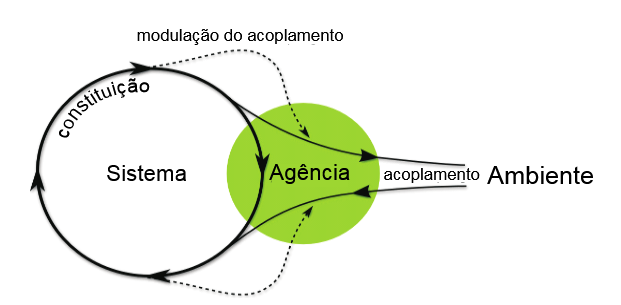
\includegraphics[width=0.5\linewidth]{figuras/modulacao.png}
    \caption{Ilustração esquemática da agência: o sistema é formado por uma rede de processos autossustentados (círculo à esquerda) em interação com o ambiente, na qual mecanismos internos de regulação modulam esse acoplamento, configurando o comportamento do agente para manter a sua identidade.\\
    \textbf{Fonte:} Adaptado de \citeonline{BarandiaranModulacao}.}
    \label{fig:modulacao}
\end{figure}

A IA Enativa, portanto, propõe uma mudança paradigmática na forma de conceber sistemas inteligentes. Em vez de projetar máquinas capazes de resolver problemas em domínios previamente especificados, o objetivo passa a ser a construção de sistemas capazes de constituir seus próprios domínios de relevância a partir de sua interação com o ambiente.

Dessa forma, um sistema artificial que incorpore simultaneamente autonomia constitutiva e adaptatividade representaria um avanço significativo em direção a modelos mais fiéis da cognição natural. Tal sistema não apenas processaria informações, mas produziria sentido, não apenas executaria tarefas, mas sustentaria sua própria existência diante das constantes ameaças impostas pelo mundo.

Em última instância, a IA Enativa sugere que a inteligência não pode ser dissociada da vida. Ser inteligente é, fundamentalmente, estar engajado em um processo contínuo de negociação com a possibilidade de deixar de existir.

\section{Fundamentação Computacional}

\subsection{Aprendizado por Reforço}
\label{subsec:aprendizado-por-reforco}

O Aprendizado por Reforço (AR) é um paradigma de aprendizado de máquina no qual um agente interage continuamente com um ambiente, tomando ações e recebendo, como consequência, sinais de feedback na forma de recompensas e novos estados. Essa interação ocorre de maneira sequencial: a cada instante, o agente observa o estado atual do ambiente, escolhe uma ação e, como resultado, o ambiente evolui para um novo estado e fornece uma recompensa associada à ação executada, conforme ilustrado na Figura~\ref{fig:rloverview}.

\begin{figure}[h!]
    \centering
    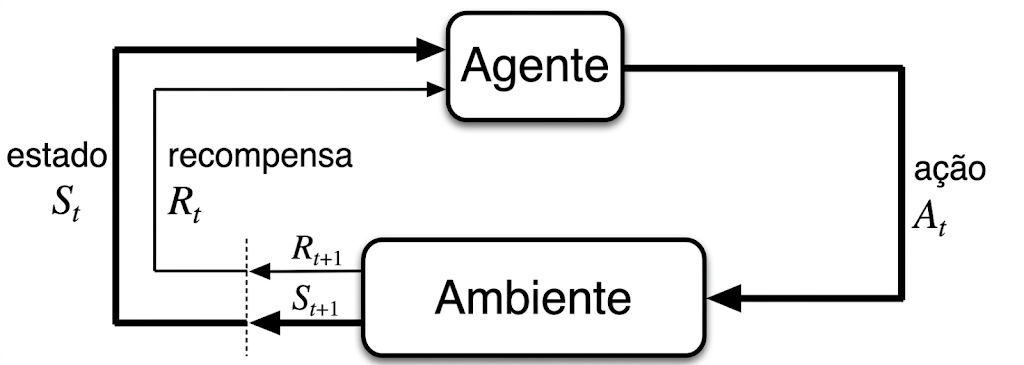
\includegraphics[width=0.5\linewidth]{figuras/rloverviewsutton.png}
    \caption{Diagrama do ciclo de interação no aprendizado por reforço. O agente observa o estado do ambiente, seleciona uma ação com base em sua política e a executa no ambiente. Como consequência, o ambiente transita para um novo estado e fornece ao agente um sinal numérico de recompensa. Esse ciclo de percepção--ação--\textit{feedback} se repete continuamente, permitindo que o agente ajuste seu comportamento ao longo do tempo de forma a maximizar a recompensa acumulada.
    \\
    \textbf{Fonte:} Adaptado de \citeonline{SuttonBarto2018}.}
    \label{fig:rloverview}
\end{figure}

O objetivo central dos algoritmos de aprendizado por reforço é aprender uma estratégia de decisão que maximize uma medida acumulada de recompensa ao longo do tempo. Diferentemente do aprendizado supervisionado, no qual pares entrada-saída são explicitamente fornecidos, no AR o agente não recebe instruções diretas sobre qual ação tomar. Em vez disso, ele deve inferir, a partir do sinal de recompensa, tentativa e erro, quais comportamentos são mais adequados, explorando o ambiente e ajustando suas decisões com base nas consequências observadas. Nos casos mais interessantes e desafiadores, as ações podem afetar não apenas a recompensa imediata, mas também a próxima situação e, por consequência, todas as recompensas subsequentes. Essas duas características, busca por tentativa e erro e recompensa atrasada, são os dois aspectos mais importantes que distinguem o aprendizado por reforço \cite{SuttonBarto2018}.

\subsubsection{Definição Matemática}

Formalmente, o problema de aprendizado por reforço é frequentemente modelado como um \textit{Processo de Decisão de Markov} (PDM), definido pela tupla:

$$
\mathcal{M} = (S, A, P, R, \gamma)
$$

\noindent em que:
\begin{itemize}
    \item $S$ é o conjunto de estados possíveis do ambiente.
    \item $A$ é o conjunto de ações disponíveis ao agente.
    \item $P(s' \mid s, a)$ é a função de transição de estados, que define a probabilidade de transitar para o estado $s'$ ao executar a ação $a$ no estado $s$. Esta função satisfaz a \textit{Propriedade de Markov}, onde a probabilidade de ir para o próximo estado depende apenas do estado atual, sendo independente da trajetória passada. Matematicamante, isso significa que:
    $$
    P(s_{t+1} \mid s_t, a_t, s_{t-1}, \dots, s_0) = P(s_{t+1} \mid s_t, a_t);
    $$
    \item $R(s, a)$ é a função de recompensa, que associa um valor escalar ao par estado-ação;
    \item $\gamma \in [0,1)$ é o fator de desconto, responsável por controlar a importância relativa das recompensas futuras no cálculo do retorno acumulado. Na equação do retorno, o termo $\gamma^k$ decai exponencialmente à medida que $k$ aumenta, fazendo com que recompensas mais distantes no tempo contribuam menos para o valor total. Dessa forma, o fator de desconto estabelece um equilíbrio entre recompensas imediatas e ganhos de longo prazo.
\end{itemize}

A dinâmica do AR ocorre em etapas discretas de tempo. Em cada instante $t$, o agente observa um estado $s_t \in S$, seleciona uma ação $a_t \in A$ de acordo com uma política $\pi$, recebe uma recompensa $r_t$ e transita para um novo estado $s_{t+1}$, como ilustrado na Figura~\ref{fig:rloverview}.

A política $\pi(a \mid s)$ define o comportamento do agente, isto é, a probabilidade de escolher a ação $a$ no estado $s$. O objetivo do agente é encontrar uma política ótima $\pi^*$ que maximize o retorno esperado, sendo este, o grande desafio dos algoritmos de aprendizagem por reforço. O retorno, por sua vez, pode ser definido em função da recompensa e do fator de desconto de recompensas futuras. Assim, o retorno a partir do tempo $t$ é definido como:

$$
G_t = \sum_{k=0}^{\infty} \gamma^k r_{t+k+1}
$$

\subsubsection{Função Valor de Estado}

Embora o objetivo do agente seja maximizar o retorno acumulado ao longo do tempo, essa quantidade, por si só, não é diretamente utilizável para a tomada de decisão em cada instante, uma vez que depende de recompensas futuras ainda desconhecidas. Dessa forma, torna-se necessário introduzir mecanismos que permitam avaliar, de maneira antecipada, a qualidade das situações nas quais o agente pode se encontrar. Nesse contexto, define-se a função valor de estado, que fornece uma medida da qualidade de um estado ao quantificar o retorno esperado a partir dele, assumindo que o agente seguirá uma determinada política $\pi$. Intuitivamente, o valor de um estado reflete o quão promissor ele é em termos de recompensas futuras, ou seja, estados com valores mais elevados indicam maior potencial de retorno, enquanto estados com valores mais baixos sugerem situações menos favoráveis. Permitindo, assim, comparar estados e orientar o agente na escolha de ações que o conduzam, de forma consistente, a regiões mais vantajosas do espaço de estados. Formalmente, a função valor de estado é definida como:
$$
V_\pi(s) = \mathbb{E}_\pi [G_t \mid s_t = s]
$$

%\subsubsection{Função Valor de Estado-Ação}

%Apesar de a função valor de estado fornecer uma medida útil da qualidade dos estados, ela não distingue explicitamente o impacto das diferentes ações que podem ser executadas a partir de um mesmo estado. Em muitos problemas, entretanto, a escolha da ação é justamente o elemento central do processo decisório, tornando necessário avaliar não apenas “onde o agente está”, mas também “o que ele faz” a partir desse estado. Para capturar essa dependência mais refinada, define-se a função valor de estado-ação, também conhecida como Q-função. Essa função associa a cada par estado-ação uma estimativa do retorno esperado, considerando que o agente executa inicialmente uma ação específica e, a partir de então, segue a política $\pi$. Intuitivamente, a função $Q_\pi(s,a)$ expressa o quão vantajoso é selecionar a ação $a$ quando o agente se encontra no estado $s$, levando em conta suas consequências futuras. Dessa forma, enquanto a função valor de estado permite comparar diferentes estados, a função valor de estado-ação possibilita comparar diretamente ações disponíveis em um mesmo estado, desempenhando um papel fundamental na derivação de políticas ótimas. Formalmente, a função valor de estado-ação é definida como:
%$$
%Q_\pi(s,a) = \mathbb{E}_\pi [G_t \mid s_t = s, a_t = a]
%$$

%\subsubsection{Equação de Bellman}

%As funções de valor definidas anteriormente fornecem uma maneira de avaliar estados e ações, mas sua utilidade prática torna-se ainda mais evidente quando observamos que elas podem ser caracterizadas de forma recursiva. Essa propriedade decorre da própria estrutura sequencial do problema de aprendizado por reforço, no qual o retorno acumulado pode ser decomposto em uma recompensa imediata somada ao retorno futuro.

%Essa ideia fundamental é formalizada por meio das equações de Bellman, que estabelecem uma relação de consistência entre o valor de um estado (ou par estado-ação) e os valores de estados subsequentes. Intuitivamente, essas equações expressam o fato de que o valor de uma situação presente deve refletir tanto o ganho imediato quanto a qualidade esperada das situações futuras que dela decorrem.

%No caso da função valor de estado, a equação de Bellman para uma política $\pi$ pode ser escrita como:
%$$
%V_\pi(s) = \sum_{a} \pi(a \mid s) \left[ R(s,a) + \gamma \sum_{s'} P(s' \mid s,a) V_\pi(s') \right]
%$$

%De maneira análoga, a função valor de estado-ação também satisfaz uma forma recursiva, dada por:
%$$
%Q_\pi(s,a) = R(s,a) + \gamma \sum_{s'} P(s' \mid s,a) \sum_{a'} \pi(a' \mid s') Q_\pi(s',a')
%$$

%Essas relações são centrais no aprendizado por reforço, pois permitem que os valores sejam estimados iterativamente a partir de suas próprias definições, constituindo a base teórica para diversos algoritmos, como métodos de programação dinâmica, aprendizado temporal-diferencial e Q-learning.

\subsection{Aprendizado por Reforço Profundo}
\label{subsec:aprendizado-por-reforco-profundo}

Embora a fundamentação matemática do Aprendizado por Reforço forneça a base para a tomada de decisão sequencial, a aplicação desses conceitos em ambientes complexos e de alta dimensionalidade enfrenta o desafio da chamada \textit{maldição da dimensionalidade}. Esse termo refere-se ao crescimento exponencial da quantidade de estados possíveis à medida que aumenta a dimensionalidade do espaço de estados. Em problemas reais, pequenas variações contínuas nas observações do ambiente podem gerar um número extremamente elevado de configurações distintas, tornando inviável armazenar explicitamente informações para cada estado possível.

Essa limitação torna-se particularmente evidente em métodos tabulares, nos quais funções de políticas são representadas por tabelas contendo estimativas associadas a cada estado. Em problemas nos quais o espaço de estados $S$ é contínuo ou composto por entradas sensoriais brutas, como pixels de imagens, o número de combinações possíveis cresce rapidamente, tornando impraticável tanto o armazenamento quanto o aprendizado eficiente dessas representações.

O Aprendizado por Reforço Profundo (ARP) \cite{mnih-2013}  resolve essa limitação ao integrar os princípios do AR com o poder de representação das Redes Neurais Profundas. Nesse paradigma, as redes neurais atuam como aproximadores de funções universais, sendo capazes de aprender representações compactas e generalizáveis a partir de dados complexos.

A principal mudança introduzida pelo ARP é a parametrização dos componentes do agente. A política $\pi$, que antes era uma distribuição de probabilidade definida em uma tabela, passa a ser representada por uma rede neural com um conjunto de parâmetros $\theta$, denotada como $\pi_\theta(a \mid s)$. O objetivo do aprendizado, portanto, desloca-se para a busca dos parâmetros $\theta$ que maximizam o retorno esperado. A figura~\ref{fig:arl} mostra o desenho esquemático de um algoritmo de ARP.

\begin{figure}[h!]
    \centering
    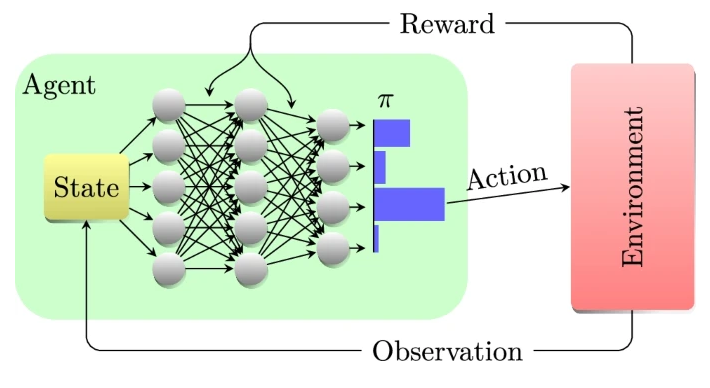
\includegraphics[width=0.8\linewidth]{figuras/arl.png}
    \caption{
        Esquema de Aprendizado por Reforço Profundo. Uma Rede Neural Profunda aprende a política $\pi$ que o agente utiliza para executar uma ação no ambiente. Uma recompensa e a informação sobre o novo estado do sistema são devolvidas ao agente, que aprimora e aprende sua política de acordo.\\
        \textbf{Fonte:} Adaptado de \citeonline{drlscheme}.
    }
    \label{fig:arl}
\end{figure}

Entretanto, para que a rede neural consiga representar adequadamente a política do agente, é necessário um mecanismo capaz de ajustar seus parâmetros internos com base nas experiências adquiridas durante a interação com o ambiente. Em redes neurais profundas, esse aprendizado ocorre por meio de um processo de otimização iterativa, no qual os parâmetros $\theta$ são atualizados de forma a minimizar uma função de perda que mede o erro entre as previsões da rede e os valores desejados.

De maneira geral, uma rede neural pode ser entendida como uma função parametrizada $f_\theta(x)$, na qual $x$ representa a entrada da rede e $\theta$ o conjunto de pesos e vieses que determinam seu comportamento. Durante o treinamento, o objetivo consiste em encontrar os valores de $\theta$ que minimizam uma função objetivo $\mathcal{L}(\theta)$, frequentemente definida em termos do erro de predição da rede.

A atualização dos parâmetros é realizada por métodos de otimização baseados em gradiente, sendo o Gradiente Descendente uma das abordagens mais utilizadas. Nesse método, calcula-se o gradiente da função de perda em relação aos parâmetros da rede,
$$
\nabla_\theta \mathcal{L}(\theta),
$$
o qual indica a direção de maior crescimento da função objetivo. Assim, para minimizar a perda, os parâmetros são atualizados iterativamente na direção oposta ao gradiente:
$$
\theta \leftarrow \theta - \alpha \nabla_\theta \mathcal{L}(\theta),
$$
em que $\alpha$ representa a taxa de aprendizado, responsável por controlar o tamanho das atualizações realizadas a cada etapa de treinamento.

O cálculo eficiente desses gradientes é realizado por meio do algoritmo de retropropagação do erro, que aplica a regra da cadeia para propagar o erro da saída da rede em direção às camadas internas, permitindo determinar a contribuição de cada parâmetro para o erro total. Dessa forma, a rede neural ajusta progressivamente suas representações internas, tornando-se capaz de aproximar funções altamente não lineares e extrair padrões relevantes dos dados observados.

No contexto do Aprendizado por Reforço Profundo, esse mecanismo de otimização é utilizado para ajustar os parâmetros da política $\pi_\theta(a \mid s)$ ou das funções de valor aproximadas pela rede neural. Assim, a experiência adquirida pelo agente durante sua interação com o ambiente é convertida em sinais de treinamento que orientam a atualização dos parâmetros $\theta$, permitindo que o comportamento do agente evolua progressivamente em direção a políticas mais eficientes.

\subsubsection{Redes Neurais Convolucionais}

Em muitos problemas de Aprendizado por Reforço Profundo, o agente não recebe como entrada estados simbólicos ou vetores de baixa dimensionalidade, mas sim dados perceptuais complexos, como imagens provenientes de câmeras ou quadros de jogos digitais. Nesses casos, torna-se necessário um mecanismo capaz de extrair automaticamente representações relevantes a partir dos dados brutos de entrada. As Redes Neurais Convolucionais \cite{cnn}, do inglês, CNNs, desempenham papel fundamental nesse contexto, sendo amplamente utilizadas em tarefas de visão computacional devido à sua capacidade de aprender características espaciais diretamente de imagens.

Diferentemente de redes totalmente conectadas, nas quais cada neurônio está ligado a todos os elementos da entrada, as CNNs exploram a estrutura espacial dos dados por meio da operação de convolução. Nessa operação, pequenos filtros percorrem a imagem realizando produtos internos locais, produzindo mapas de ativação que destacam padrões específicos presentes na entrada. Formalmente, a convolução discreta bidimensional entre uma entrada $I$ e um filtro $K$ pode ser expressa como:
$$
S(i,j) = (I \circledast K)(i,j) = \sum_m \sum_n I(i-m, j-n)K(m,n),
$$
em que $S(i,j)$ representa o valor produzido na posição $(i,j)$ do mapa de características resultante.

Durante o treinamento, os valores dos filtros convolucionais são aprendidos automaticamente pela rede neural por meio da retropropagação do erro. Dessa forma, diferentes filtros passam a responder a diferentes padrões visuais presentes na imagem. Nas primeiras camadas da rede, os filtros tendem a detectar características simples, como bordas, texturas e contrastes. À medida que a informação se propaga para camadas mais profundas, a rede combina essas características elementares para representar estruturas progressivamente mais complexas, como formas, objetos ou regiões semanticamente relevantes.

Outra propriedade importante das CNNs é o compartilhamento de parâmetros. Como o mesmo filtro é aplicado em diferentes regiões da imagem, o número de parâmetros necessários torna-se significativamente menor em comparação com redes totalmente conectadas. Além de reduzir o custo computacional, essa característica permite que a rede desenvolva invariância translacional parcial, isto é, a capacidade de reconhecer padrões independentemente de sua posição exata na imagem.

Frequentemente, as camadas convolucionais são combinadas com operações de subamostragem (\textit{pooling}), responsáveis por reduzir a dimensionalidade espacial dos mapas de ativação e aumentar a robustez das representações aprendidas. Em particular, operações como \textit{max-pooling} preservam apenas as ativações mais relevantes de uma região local, contribuindo para a redução de ruído e para a generalização do modelo. A arquitetura geral de uma CNN pode ser visto na figura~\ref{fig:cnn}.

\begin{figure}
    \centering
    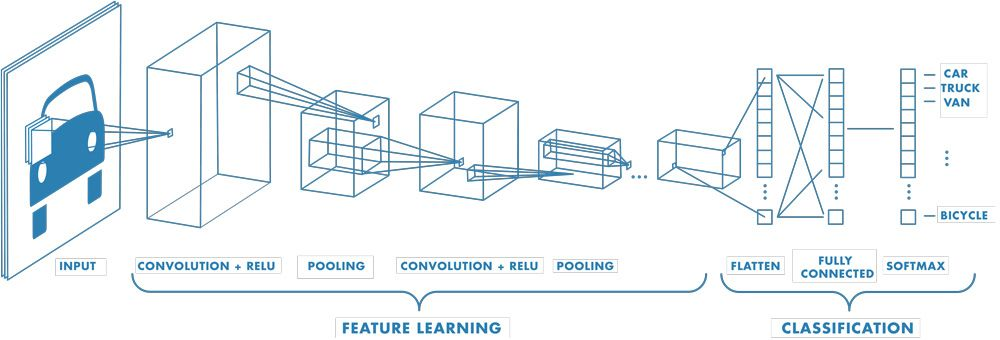
\includegraphics[width=0.75\linewidth]{figuras/cnn.png}
    \caption{Representação esquemática de uma arquitetura CNN, destacando os blocos de extração de características (convolução e pooling) e os blocos de classificação final (camadas densas e softmax).\\
    \textbf{Fonte:} Adaptado de \citeonline{cnn-image}.}
    \label{fig:cnn}
\end{figure}

No caso do ARP, a CNN atua como um mecanismo de percepção capaz de transformar imagens de alta dimensionalidade em representações compactas e semanticamente relevantes, que posteriormente são utilizadas pela política do agente para a tomada de decisão.

\subsection{Aprendizado Contínuo}

Dentro dos algoritmos de Aprendizado por Reforço, é possível distinguir dois tipos principais: métodos \textit{on-policy} e \textit{off-policy}. Segundo \citeonline{SuttonBarto2018}, a principal diferença entre essas abordagens está na relação entre a política utilizada para gerar experiências no ambiente e a política efetivamente atualizada durante o aprendizado. Métodos \textit{on-policy} avaliam ou aprimoram a mesma política responsável pela interação atual do agente com o ambiente. Já métodos \textit{off-policy} permitem aprender uma política-alvo distinta daquela utilizada para coletar experiências, desacoplando a política de comportamento da política que está sendo otimizada.

Em algoritmos \textit{on-policy}, a política utilizada para agir no ambiente é exatamente a mesma política que está sendo aprendida. Isso significa que o agente adapta seu comportamento diretamente a partir das experiências produzidas por sua política atual. O processo de aprendizado permanece continuamente alinhado ao modo como o agente percebe, age e interage no ambiente naquele momento específico.

Por outro lado, métodos \textit{off-policy} permitem que o aprendizado utilize experiências geradas por políticas diferentes da política atual do agente. Assim, a política-alvo pode continuar sendo otimizada utilizando dados coletados anteriormente, experiências produzidas sob estratégias mais exploratórias ou até trajetórias geradas por outros agentes. Dessa forma, o aprendizado deixa de depender exclusivamente da política atualmente em execução.

%Uma analogia simples para compreender essa diferença é pensar no processo de aprender a dirigir. Em uma abordagem \textit{on-policy}, a pessoa aprende enquanto efetivamente dirige: ela realiza ações, observa imediatamente suas consequências e ajusta continuamente sua maneira de conduzir o veículo. O aprendizado emerge diretamente da interação presente entre motorista e ambiente.

%Já em uma abordagem \textit{off-policy}, além da experiência direta ao volante, a pessoa também pode aprender observando gravações de outras pessoas dirigindo, analisando trajetórias passadas ou estudando estratégias diferentes daquelas que ela própria executa naquele momento. Nesse caso, o aprendizado não está necessariamente vinculado à política atual de comportamento, mas pode incorporar experiências produzidas sob diferentes modos de ação.

Essa distinção possui implicações importantes quando analisada sob a perspectiva da IA Enativa. Em abordagens \textit{on-policy}, o aprendizado ocorre de forma fortemente acoplada à política atualmente incorporada pelo agente durante sua interação com o ambiente. A política utilizada para perceber, agir e explorar o mundo é a mesma política continuamente transformada pela experiência vivida. Assim, cognição e adaptação emergem conjuntamente da dinâmica de interação situada entre agente e ambiente.

Sob a ótica da IA Enativa, esse acoplamento reforça a ideia de que o conhecimento não é simplesmente armazenado ou processado de maneira abstrata, mas construído continuamente a partir da própria atividade do agente no mundo. O agente age sobre o ambiente, sofre diretamente as consequências de suas ações e modifica seu comportamento com base nos efeitos produzidos por essa interação contínua. Dessa forma, o aprendizado não aparece como um processo separado da ação, mas como parte integrante do ciclo contínuo de percepção, ação e adaptação, no qual a própria experiência vivida transforma continuamente a política utilizada pelo agente.

Em contraste, métodos \textit{off-policy} introduzem uma separação parcial entre a política responsável pela experiência atual e a política efetivamente aprendida. Embora isso aumente significativamente a eficiência amostral e permita maior reutilização de experiências, o processo de adaptação torna-se menos diretamente dependente da interação presente do agente com o ambiente. Sob a perspectiva enativa, isso reduz parcialmente o vínculo imediato entre cognição e ação situada, aproximando o aprendizado de um processo mais mediado pela reutilização e processamento de experiências previamente coletadas.


\subsubsection{Métodos de Gradiente de Política}

No âmbito dos métodos \textit{on-policy}, uma das primeiras abordagens consolidadas são os métodos de gradiente de política (\textit{Policy Gradient Methods}) \cite{policygradient}. Diferentemente de métodos baseados em função valor, nos quais o agente aprende indiretamente uma política a partir da estimativa de valores de estados ou ações, os métodos de gradiente de política buscam otimizar diretamente a própria política do agente.

Nessa abordagem, a política é parametrizada por um conjunto de parâmetros $\theta$, geralmente representados pelos pesos de uma rede neural, sendo denotada por $\pi_\theta(a|s)$. Essa política define uma distribuição de probabilidade sobre as ações possíveis em cada estado do ambiente. O objetivo do aprendizado consiste em encontrar os parâmetros $\theta$ que maximizem o retorno esperado obtido pelo agente ao interagir com o ambiente. Formalmente, deseja-se maximizar:
$$
J(\pi_\theta) = \mathbb{E}_{\tau \sim \pi_\theta}[R(\tau)],
$$

em que $\tau$ representa uma trajetória gerada pela interação entre agente e ambiente. Uma trajetória corresponde à sequência de estados, ações e recompensas observadas durante um episódio de interação, podendo ser representada por:

$$
\tau = (s_0, a_0, r_1, s_1, a_1, r_2, \dots, s_T).
$$

O termo $R(\tau)$ representa o retorno acumulado ao longo dessa trajetória. Assim, o objetivo do agente é ajustar sua política de modo que trajetórias com maiores retornos tornem-se mais prováveis.

Para isso, os métodos de gradiente de política utilizam o gradiente da função objetivo em relação aos parâmetros da política:
$$
\nabla_\theta J(\pi_\theta).
$$

A ideia central consiste em aumentar a probabilidade de ações que levaram a retornos elevados e reduzir a probabilidade de ações associadas a retornos menores. Intuitivamente, se determinadas escolhas resultaram em consequências favoráveis ao agente, a política deve ser atualizada para tornar tais ações mais prováveis em situações semelhantes futuras.

A partir do chamado Teorema do Gradiente da Política, é possível escrever o gradiente da política na forma:
$$
\nabla_\theta J(\pi_\theta)
=
\mathbb{E}_{\tau \sim \pi_\theta}
\left[
\sum_{t=0}^{T}
\nabla_\theta \log \pi_\theta(a_t|s_t)
R(\tau)
\right].
$$

Apesar de estabelecerem uma formulação teórica geral para otimização direta de políticas parametrizadas, métodos de gradiente de política apresentam limitações importantes na prática. Pequenas alterações nos parâmetros podem gerar mudanças significativas no comportamento da política, tornando o treinamento instável. De forma análoga, um pequeno ajuste na direção de um veículo em alta velocidade pode alterar drasticamente sua trajetória. Em políticas parametrizadas por redes neurais, pequenas atualizações nos parâmetros podem modificar significativamente as probabilidades das ações executadas, fazendo com que o comportamento do agente varie abruptamente entre diferentes etapas do treinamento. Além disso, as estimativas do gradiente frequentemente apresentam alta variância, exigindo grande quantidade de interações com o ambiente para obtenção de aprendizado estável e eficiente.

\subsubsection{Trust Region Policy Optimization}

As limitações observadas nos métodos clássicos de gradiente de política motivaram o desenvolvimento de abordagens mais estáveis para atualização da política. Embora esses métodos permitam otimizar diretamente o comportamento do agente, pequenas atualizações nos parâmetros podem provocar mudanças abruptas na distribuição de ações da política, comprometendo o desempenho aprendido anteriormente. Em muitos casos, uma única atualização inadequada é suficiente para fazer o agente perder comportamentos que já haviam sido aprendidos.

Diante desse problema, o \textit{Trust Region Policy Optimization} (TRPO) \cite{trpo} introduz a ideia de limitar explicitamente o quanto a política pode mudar a cada etapa de treinamento. Em vez de apenas seguir a direção do gradiente de maior recompensa esperada, o TRPO busca garantir que a nova política permaneça suficientemente próxima da política anterior. Assim, o agente continua aprendendo, mas de maneira mais controlada e estável.

Formalmente, o TRPO procura maximizar uma função objetivo associada à vantagem esperada da nova política em relação à política antiga, ao mesmo tempo em que impõe uma restrição sobre a divergência entre ambas:

$$
\theta_{k+1}
=
\arg\max_{\theta}
\mathcal{L}(\theta_k,\theta)
\quad
\text{sujeito a}
\quad
\bar{D}_{KL}(\theta \,\|\, \theta_k) \leq \delta.
$$

Nesse contexto, $\mathcal{L}(\theta_k,\theta)$ representa uma aproximação do ganho esperado ao atualizar a política, enquanto $\bar{D}_{KL}$ corresponde à divergência de Kullback-Leibler média entre a política antiga e a nova política. Essa divergência atua como uma medida de diferença entre distribuições de probabilidade, permitindo controlar o quanto o comportamento do agente pode variar entre duas atualizações consecutivas.

Intuitivamente, o TRPO impede que o agente ``mude de ideia'' de maneira excessivamente brusca. Mesmo que o gradiente indique uma direção potencialmente vantajosa, o algoritmo restringe o tamanho do passo de atualização, garantindo que a política evolua gradualmente. Isso reduz colapsos repentinos de desempenho e produz um processo de aprendizado mais estável.

Apesar de suas vantagens, o TRPO apresenta elevada complexidade computacional. O método exige resolver um problema de otimização restrita relativamente sofisticado, envolvendo aproximações de segunda ordem e cálculos relacionados à matriz Hessiana da divergência KL. Na prática, isso torna sua implementação mais difícil e computacionalmente mais custosa quando comparada a métodos mais simples de gradiente de política.

Ainda assim, o TRPO representou um avanço importante na evolução dos métodos \textit{on-policy}, ao introduzir mecanismos explícitos de estabilidade no processo de atualização da política. Suas ideias serviram posteriormente de base para algoritmos mais simples e eficientes, como o \textit{Proximal Policy Optimization} (PPO), que preserva a intuição central do TRPO, mas reduz significativamente sua complexidade computacional.

\subsubsection{Proximal Policy Optimization}
\label{subsubsec:ppo}

O \textit{Proximal Policy Optimization} (PPO) \cite{ppo} surge como uma evolução natural das ideias introduzidas pelo TRPO. Assim como seu predecessor, o PPO busca evitar que atualizações excessivamente grandes da política provoquem degradações abruptas de desempenho. Entretanto, em vez de resolver um problema de otimização restrita complexo, o PPO adota uma estratégia significativamente mais simples e eficiente, baseada em um mecanismo denominado \textit{clipping}.

A motivação central permanece a mesma: permitir que o agente aprenda continuamente sem alterar drasticamente seu comportamento entre duas atualizações consecutivas. Em métodos clássicos de gradiente de política, uma atualização muito intensa pode fazer com que a política passe a escolher ações completamente diferentes das anteriores, destruindo comportamentos úteis já aprendidos. O PPO procura limitar esse problema de forma prática e computacionalmente eficiente.

Formalmente, o algoritmo compara a nova política $\pi_\theta$ com a política anterior $\pi_{\theta_{\text{old}}}$ por meio da razão:

$$
r_t(\theta)
=
\frac{\pi_\theta(a_t \mid s_t)}
{\pi_{\theta_{\text{old}}}(a_t \mid s_t)}.
$$

Essa razão mede o quanto a nova política aumentou ou reduziu a probabilidade de executar a ação $a_t$ no estado $s_t$. Valores próximos de $1$ indicam poucas mudanças entre as políticas, enquanto valores muito maiores ou menores indicam alterações mais agressivas no comportamento do agente.

A função objetivo do PPO incorpora então um mecanismo de \textit{clipping}, definido por:

$$
L^{\text{CLIP}}(\theta)
=
\mathbb{E}_t
\left[
\min
\left(
r_t(\theta)\hat{A}_t,
\;
\text{clip}(r_t(\theta),1-\epsilon,1+\epsilon)\hat{A}_t
\right)
\right],
$$

\noindent em que $\hat{A}_t$ representa a vantagem estimada da ação executada. Intuitivamente, essa vantagem mede o quanto uma ação produziu resultados melhores ou piores do que o esperado pela política atual. Em geral, a vantagem é estimada pela diferença entre o retorno efetivamente obtido após executar a ação e o valor esperado para o estado correspondente, podendo ser expressa por:

$$
\hat{A}_t \approx \hat{R}_t - V(s_t),
$$

\noindent onde $\hat{R}_t$ representa o retorno acumulado observado a partir do instante $t$, enquanto $V(s_t)$ corresponde à estimativa de valor do estado $s_t$, isto é, a recompensa esperada ao seguir a política atual a partir desse estado. Dessa forma, vantagens positivas indicam ações que produziram resultados melhores do que o esperado, enquanto vantagens negativas indicam ações menos vantajosas. Já o parâmetro $\epsilon$ define o limite permitido para a variação da política entre atualizações consecutivas.

Embora essa expressão matemática pareça complexa, sua ideia intuitiva é relativamente simples. O PPO recompensa mudanças que melhoram o desempenho da política, mas impede que essas mudanças se tornem excessivamente grandes. O mecanismo de \textit{clipping} funciona como um limitador de segurança: quando a nova política tenta alterar demais a probabilidade de determinadas ações, o algoritmo interrompe o benefício adicional dessa mudança.

Por combinar simplicidade computacional, estabilidade de treinamento e boa eficiência empírica, o PPO tornou-se um dos algoritmos \textit{on-policy} mais utilizados em Aprendizado por Reforço Profundo. Sua capacidade de manter um equilíbrio entre exploração, aprendizado contínuo e estabilidade fez com que ele fosse amplamente adotado em aplicações envolvendo ambientes complexos e de alta dimensionalidade.

\subsection{Exploração, Motivação Intrínseca e Curiosidade}

Um dos principais desafios no Aprendizado por Reforço é o chamado dilema de exploração versus explotação. Esse dilema consiste em decidir entre duas estratégias conflitantes: \textit{explotar}, isto é, aproveitar o conhecimento atual para maximizar recompensas imediatas ou \textit{explorar} o ambiente em busca de novas informações que possam levar a recompensas maiores no futuro. Enquanto a explotação tende a ser segura e eficiente no curto prazo, a exploração é essencial para evitar soluções sub-ótimas e descobrir estados potencialmente mais vantajosos.

Esse problema se torna particularmente crítico em ambientes com recompensas esparsas, onde sinais de recompensa são raros e difíceis de encontrar. Nessas condições, agentes puramente orientados à explotação frequentemente falham, pois não conseguem coletar informação suficiente para aprender políticas eficazes. Assim, mecanismos que incentivem a exploração tornam-se fundamentais.

\subsubsection{Recompensa Intrínseca}

Uma forma de compreender esse desafio é por meio da distinção entre \textit{motivação intrínseca} e \textit{motivação extrínseca}, amplamente estudada na literatura psicológica \cite{intrinsic}. Motivação intrínseca refere-se à realização de uma atividade por seu valor inerente, isto é, pelo interesse, curiosidade ou satisfação associada à própria execução da tarefa. Em contraste, a motivação extrínseca está associada à realização de uma atividade como meio para atingir um objetivo externo, como recompensas, reconhecimento ou evitar punições.

Essa distinção é particularmente relevante porque, embora ambas as formas de motivação possam levar à execução de uma mesma ação, elas diferem fundamentalmente em sua origem e nos comportamentos que incentivam. Enquanto a motivação extrínseca é guiada por consequências externas ao agente, a motivação intrínseca está relacionada a uma propensão natural à exploração, aprendizado e assimilação de novas informações . Em humanos, por exemplo, comportamentos exploratórios frequentemente emergem mesmo na ausência de recompensas explícitas, sendo impulsionados por curiosidade e interesse.

No contexto do Aprendizado por Reforço, essa distinção pode ser reinterpretada de forma análoga: recompensas extrínsecas correspondem aos sinais fornecidos diretamente pelo ambiente, enquanto recompensas intrínsecas são introduzidas artificialmente no agente como forma de incentivar comportamentos desejáveis, como a exploração de estados desconhecidos. Essa perspectiva tem motivado o desenvolvimento de diversas técnicas que aumentam a função de recompensa com sinais internos ao agente, visando superar limitações impostas por recompensas esparsas ou pouco informativas. Com isso, a recompensa total pode ser definida como:
$$ 
r_t = r_t^{\text{ext}} + r_t^{\text{int}},
$$
onde $r_t^{\text{ext}}$ é a recompensa extrínseca e $r_t^{\text{int}}$ representa a recompensa intrínseca. 

Na prática, a recompensa intrínseca pode ser implementada de diferentes maneiras, a depender de quais aspectos do processo de aprendizado se deseja enfatizar. Uma forma de implementar esse tipo de sinal é por meio da noção de \textit{curiosidade} \cite{icm}. Nesse contexto, a curiosidade pode ser entendida como a tendência do agente em buscar experiências que revelem limitações em seu conhecimento atual, isto é, situações nas quais sua capacidade de previsão ou compreensão ainda é insuficiente. Dessa forma, estados que são difíceis de prever ou que diferem significativamente da experiência prévia do agente tornam-se mais atrativos.

A partir dessa perspectiva, a curiosidade pode ser formalizada como um tipo de recompensa intrínseca, na qual o agente recebe um bônus adicional ao interagir com estados considerados novos ou informativos. Esse tipo de formulação permite traduzir o comportamento exploratório em um sinal quantitativo, que pode ser incorporado diretamente à função de recompensa.

\subsubsection{ Random Network Destillation}
\label{subsubsec:rnd}

Dentro desse contexto, destaca-se o método de \textit{Random Network Distillation} (RND) \cite{rnd}, proposto como uma forma simples e eficiente de incentivar a exploração em ambientes de alta dimensionalidade. A ideia central do RND é utilizar o erro de predição como medida de novidade.

O método consiste em duas redes neurais: uma rede alvo fixa, inicializada aleatoriamente, e uma rede preditora treinável. Em geral, ambas possuem a mesma arquitetura, normalmente implementada por redes neurais convolucionais quando as observações do ambiente são imagens. Nesse caso, as camadas convolucionais são responsáveis por extrair características espaciais relevantes da entrada, enquanto camadas totalmente conectadas projetam essas características em um espaço latente de menor dimensionalidade.

A rede alvo possui parâmetros fixos, inicializados aleatoriamente no início do treinamento e mantidos inalterados ao longo de toda a execução do algoritmo. Dessa forma, ela define uma função determinística que mapeia observações do ambiente para representações vetoriais em um espaço de características. Já a rede preditora possui parâmetros treináveis e tem como objetivo aproximar a saída produzida pela rede alvo para uma determinada observação.

O treinamento da rede preditora é realizado por aprendizado supervisionado, utilizando como alvo a saída da rede fixa. Assim, a cada nova observação $s_t$, a rede preditora ajusta seus parâmetros por meio de descida do gradiente, minimizando o erro quadrático médio (\textit{Mean Squared Error} -- MSE) entre sua saída e a saída produzida pela rede alvo. Esse processo é ilustrado na Figura~\ref{fig:rnd}.

\begin{figure}[h!]
    \centering
    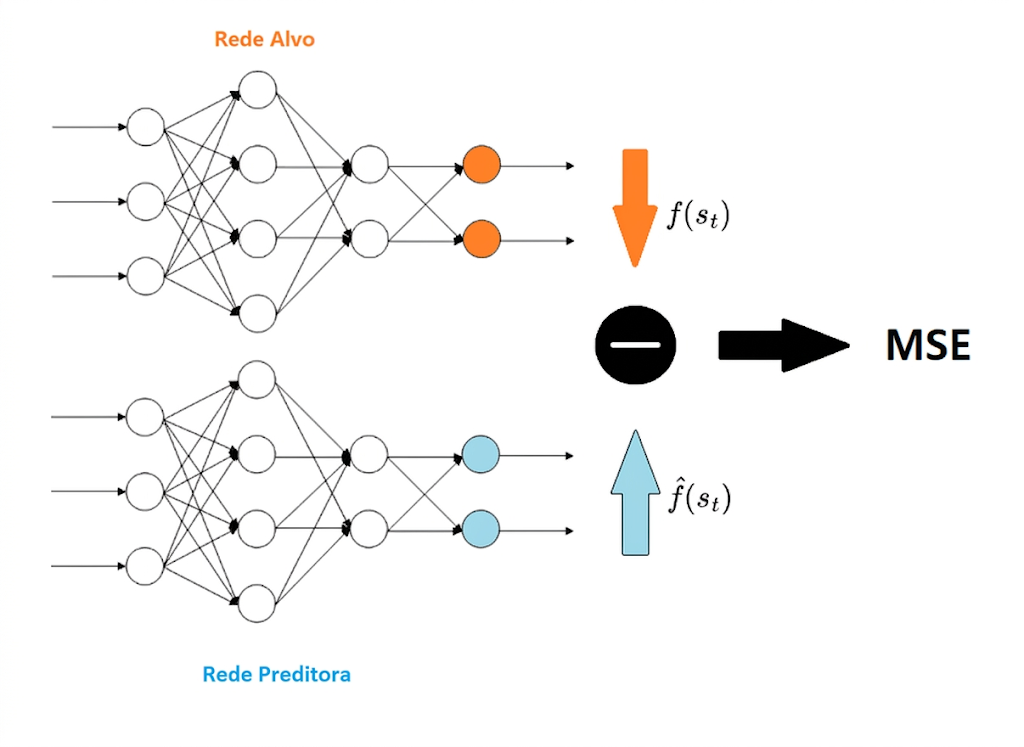
\includegraphics[width=0.8\linewidth]{figuras/rnd.png}
    \caption{Arquitetura do método \textit{Random Network Distillation} (RND). O erro quadrático médio (MSE) entre a saída da Rede Alvo fixa ($f(s_t)$) e a Rede Preditora treinável ($\hat{f}(s_t)$) é utilizado como sinal de curiosidade ou recompensa intrínseca.}
    \label{fig:rnd}
\end{figure}

A intuição por trás dessa abordagem é que estados frequentemente visitados terão seus padrões bem aprendidos pela rede preditora, resultando em baixo erro de predição. Por outro lado, estados novos ou raros produzirão erros elevados, gerando um forte sinal de recompensa intrínseca que incentiva o agente a explorá-los.

Em síntese, a introdução de mecanismos de curiosidade e motivação intrínseca, como o RND, representa um avanço significativo na resolução do dilema exploração-explotação, permitindo que agentes aprendam de forma mais eficiente em ambientes desafiadores e pouco informativos.

\subsection{Análise Visual da Política Aprendida}

Embora mecanismos de motivação intrínseca, como o RND, promovam uma exploração mais eficiente do ambiente, eles também tornam o comportamento do agente mais difícil de interpretar. Isso ocorre porque a política aprendida passa a ser influenciada não apenas por recompensas extrínsecas explícitas, mas também por sinais internos de curiosidade, cuja dinâmica pode não ser imediatamente evidente. Nesse contexto, compreender por que o agente toma determinadas decisões torna-se um desafio fundamental.

Modelos baseados em redes neurais profundas, frequentemente utilizados para representar políticas em Aprendizado por Reforço, são conhecidos por seu alto poder de representação, mas também por sua baixa interpretabilidade. Esses modelos operam como verdadeiras ``caixas pretas'', nas quais a relação entre entrada (estado) e saída (ação) não é facilmente compreendida. Assim, mesmo quando o agente apresenta um bom desempenho, torna-se difícil identificar quais aspectos do ambiente estão sendo considerados relevantes para a tomada de decisão.

Uma abordagem promissora para lidar com esse problema é o uso de técnicas de Inteligência Artificial Explicável (XAI), em particular métodos de visualização que permitem identificar regiões da entrada responsáveis por uma determinada decisão.

\subsubsection{Gradient-weighted Class Activation Mapping}
\label{subsubsec:gradcam}

Uma das abordagens iniciais para promover interpretabilidade em redes convolucionais é o \textit{Class Activation Mapping} (CAM) \cite{cam}, que permite identificar regiões da imagem relevantes para a predição de uma determinada classe. O CAM baseia-se na combinação linear dos mapas de ativação da última camada convolucional, ponderados pelos pesos associados à camada de classificação. Apesar de sua simplicidade e interpretabilidade direta, esse método apresenta limitações importantes, uma vez que requer modificações específicas na arquitetura da rede, como a substituição de camadas totalmente conectadas por operações de \textit{global average pooling}. Essa restrição dificulta sua aplicação em modelos já treinados ou em arquiteturas mais complexas.

Com o objetivo de superar essas limitações, foi proposto o método \textit{Gradient-weighted Class Activation Mapping} (Grad-CAM) \cite{gradcam}, que generaliza a ideia do CAM ao utilizar informações de gradiente para estimar a importância dos mapas de ativação, tornando possível sua aplicação em uma ampla variedade de arquiteturas sem a necessidade de alterações estruturais ou re-treinamento do modelo, a visão panorâmica do método pode ser vista na figura~\ref{fig:gradcam}.

\begin{figure}[h!]
    \centering
    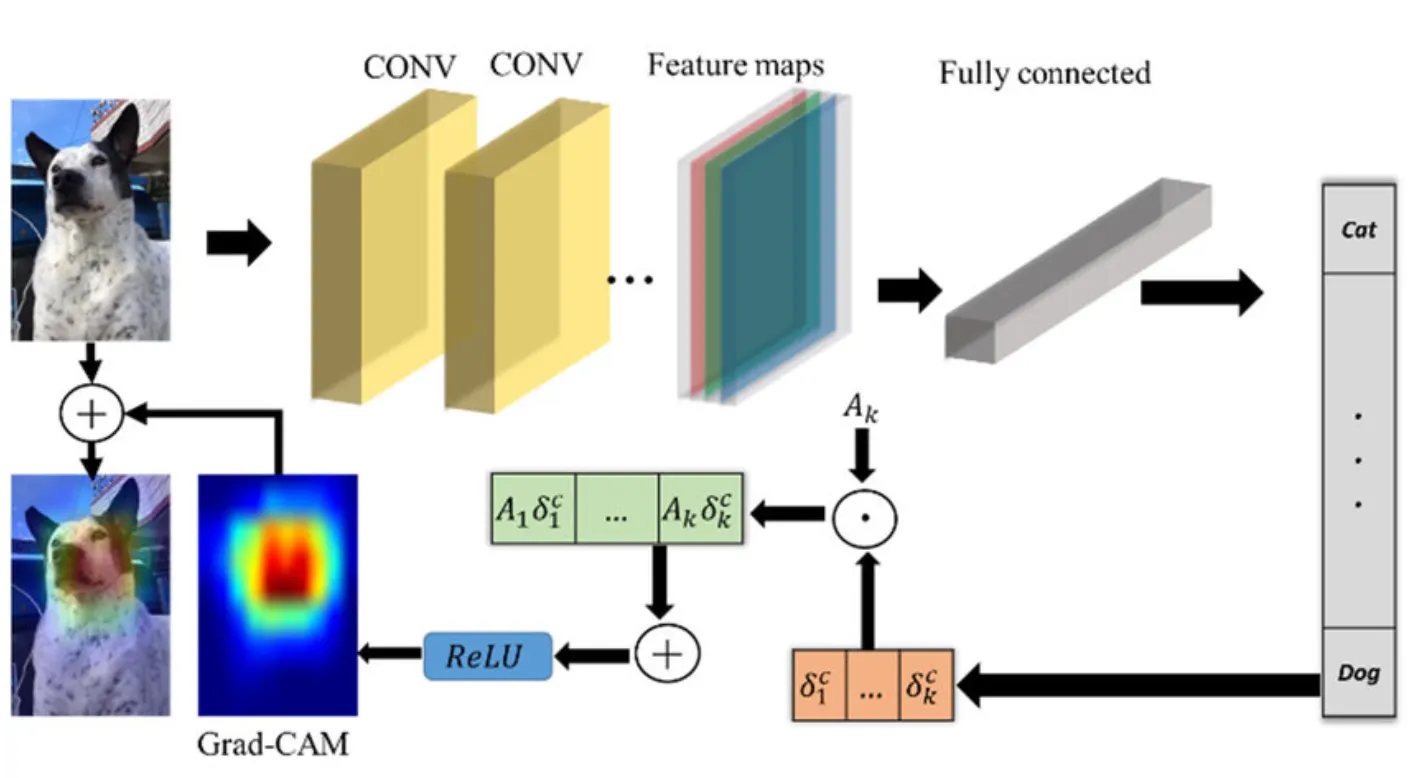
\includegraphics[width=0.75\linewidth]{figuras/gradcam.png}
    \caption{Visão panorâmica do método Grad-CAM. A ilustração detalha o fluxo de processamento onde informações de gradiente são utilizadas para ponderar os mapas de características das camadas convolucionais, resultando na geração de um mapa de calor que destaca as regiões relevantes da imagem de entrada para a classificação final.\\
     \textbf{Fonte:} Adaptado de \citeonline{gradcamimage-site}.}
    \label{fig:gradcam}
\end{figure}

O Grad-CAM baseia-se na análise dos gradientes do escore de saída de uma classe (ou, no contexto de Aprendizado por Reforço, de uma ação ou valor associado) em relação aos mapas de ativação de uma camada convolucional. Especificamente, os gradientes são utilizados para estimar a importância de cada mapa de ativação na decisão final do modelo. Esses valores de importância são então utilizados para ponderar linearmente os mapas de ativação, gerando um mapa de calor que indica as regiões da entrada mais relevantes para a decisão considerada.

Formalmente, seja $y^c$ o escore associado a uma saída de interesse $c$, e $A^k$ o $k$-ésimo mapa de ativação de uma camada convolucional. A importância de cada mapa é dada por:
$$
\alpha_k^c = \frac{1}{Z} \sum_i \sum_j \frac{\partial y^c}{\partial A_{ij}^k},
$$
onde $Z$ representa o número total de elementos no mapa. Em outras palavras, investiga-se como pequenas variações nessas representações internas impactam o valor associado à classe considerada. Regiões cuja variação provoca maior alteração no escore são interpretadas como mais relevantes para a decisão do modelo e são destacadas com maior intensidade, enquanto regiões com pouca ou nenhuma influência apresentam menor intensidade. O mapa de ativação final é então obtido pela combinação linear dos scores com os mapas de ativação:
$$
L_{\text{Grad-CAM}}^c = \text{ReLU}\left( \sum_k \alpha_k^c A^k \right).
$$

A aplicação da função ReLU garante que apenas as contribuições positivas, isto é, aquelas que aumentam o escore da saída de interesse, sejam consideradas, resultando em um mapa de calor que destaca evidências favoráveis à decisão do modelo.

No contexto de aprendizagem por reforço, o Grad-CAM pode ser utilizado para analisar visualmente a política aprendida pelo agente. Ao destacar quais regiões do estado observado influenciam determinadas ações, torna-se possível investigar como o agente está utilizando as informações do ambiente, bem como avaliar o impacto de mecanismos de exploração, como o RND, no processo de tomada de decisão. Dessa forma, a combinação entre motivação intrínseca e interpretabilidade contribui não apenas para o desempenho do agente, mas também para uma compreensão mais profunda de seu comportamento.